% This is "sig-alternate.tex" V2.0 May 2012
% This file should be compiled with V2.5 of "sig-alternate.cls" May 2012
%
% This example file demonstrates the use of the 'sig-alternate.cls'
% V2.5 LaTeX2e document class file. It is for those submitting
% articles to ACM Conference Proceedings WHO DO NOT WISH TO
% STRICTLY ADHERE TO THE SIGS (PUBS-BOARD-ENDORSED) STYLE.
% The 'sig-alternate.cls' file will produce a similar-looking,
% albeit, 'tighter' paper resulting in, invariably, fewer pages.
%
% ----------------------------------------------------------------------------------------------------------------
% This .tex file (and associated .cls V2.5) produces:
%       1) The Permission Statement
%       2) The Conference (location) Info information
%       3) The Copyright Line with ACM data
%       4) NO page numbers
%
% as against the acm_proc_article-sp.cls file which
% DOES NOT produce 1) thru' 3) above.
%
% Using 'sig-alternate.cls' you have control, however, from within
% the source .tex file, over both the CopyrightYear
% (defaulted to 200X) and the ACM Copyright Data
% (defaulted to X-XXXXX-XX-X/XX/XX).
% e.g.
% \CopyrightYear{2007} will cause 2007 to appear in the copyright line.
% \crdata{0-12345-67-8/90/12} will cause 0-12345-67-8/90/12 to appear in the copyright line.
%
% ---------------------------------------------------------------------------------------------------------------
% This .tex source is an example which *does* use
% the .bib file (from which the .bbl file % is produced).
% REMEMBER HOWEVER: After having produced the .bbl file,
% and prior to final submission, you *NEED* to 'insert'
% your .bbl file into your source .tex file so as to provide
% ONE 'self-contained' source file.
%
% ================= IF YOU HAVE QUESTIONS =======================
% Questions regarding the SIGS styles, SIGS policies and
% procedures, Conferences etc. should be sent to
% Adrienne Griscti (griscti@acm.org)
%
% Technical questions _only_ to
% Gerald Murray (murray@hq.acm.org)
% ===============================================================
%
% For tracking purposes - this is V2.0 - May 2012

\documentclass{sig-alternate}

%preambles
\usepackage{alltt                                    % I like these
          , multirow
          , booktabs
          , listings
          , graphicx
          ,float
	,cite
          ,verbatim
         ,mathtools
	,url
	,amsmath
}
\usepackage[table]{xcolor}
\usepackage[numbers]{natbib}     % this is a better citation system
\usepackage{syntax}
\usepackage{algorithmic, algorithm}
\usepackage{enumitem}
\usepackage{threeparttable}

\usepackage{expl3}
\ExplSyntaxOn
\newcommand\latinabbrev[1]{
  \peek_meaning:NTF . {% Same as \@ifnextchar
    #1\@}%
  { \peek_catcode:NTF a {% Check whether next char has same catcode as \'a, i.e., is a letter
      #1., \@ }%
    {#1., \@}}}
\ExplSyntaxOff

%switch case statement
\newcommand{\SWITCH}[1]{\STATE \textbf{switch} (#1)}
\newcommand{\ENDSWITCH}{\STATE \textbf{end switch}}
\newcommand{\CASE}[1]{\STATE \textbf{case} #1\textbf{:} \begin{ALC@g}}
\newcommand{\ENDCASE}{\end{ALC@g}}
\newcommand{\CASELINE}[1]{\STATE \textbf{case} #1\textbf{:} }
\newcommand{\DEFAULT}{\STATE \textbf{default:} \begin{ALC@g}}
\newcommand{\ENDDEFAULT}{\end{ALC@g}}
\newcommand{\DEFAULTLINE}[1]{\STATE \textbf{default:} }
%switch case statement
\let\footnotesize\scriptsize


\newsavebox{\supbox}% Superscript box
\newcommand{\bsup}{\begin{lrbox}{\supbox}$\tt\scriptstyle}% Superscript begin
\newcommand{\esup}{$\end{lrbox}{}^{\usebox{\supbox}}}% Superscript end
\def\eg{\latinabbrev{e.g}}
\def\ie{\latinabbrev{i.e}}

\renewcommand{\labelenumi}{(\alph{enumi})}

\definecolor{lightpurple}{rgb}{0.8,0.8,1}
\definecolor{codebg}{RGB}{255,255,255}
\definecolor{commentcolor}{RGB}{11,140,11}
%listing settings
\lstset{ 
    language=java, % choose the language of the code
    basicstyle=\fontfamily{pcr}\selectfont\scriptsize\color{black},
    keywordstyle=\color{blue}\bfseries, % style for keywords
   commentstyle=\color{commentcolor},
    numbers=none, % where to put the line-numbers
    numberstyle=\tiny, % the size of the fonts that are used for the line-numbers     
    backgroundcolor=\color{codebg},
    showspaces=false, % show spaces adding particular underscores
    showstringspaces=false, % underline spaces within strings
    showtabs=false, % show tabs within strings adding particular underscores
    frame=single, % adds a frame around the code
    tabsize=2, % sets default tabsize to 2 spaces
    rulesepcolor=\color{gray},
    %rulecolor=\color{black},
    captionpos=b, % sets the caption-position to bottom
    breaklines=true, % sets automatic line breaking
    breakatwhitespace=false, 
}




\begin{document}
%
% --- Author Metadata here ---
\conferenceinfo{ICSE}{'2013, Hyderabad India}
%\CopyrightYear{2007} % Allows default copyright year (20XX) to be over-ridden - IF NEED BE.
%\crdata{0-12345-67-8/90/01}  % Allows default copyright data (0-89791-88-6/97/05) to be over-ridden - IF NEED BE.
% --- End of Author Metadata ---

\title{Code Quality Analysis of StackOverflow Code Examples for Reusability: An Exploratory Study}
%
% You need the command \numberofauthors to handle the 'placement
% and alignment' of the authors beneath the title.
%
% For aesthetic reasons, we recommend 'three authors at a time'
% i.e. three 'name/affiliation blocks' be placed beneath the title.
%
% NOTE: You are NOT restricted in how many 'rows' of
% "name/affiliations" may appear. We just ask that you restrict
% the number of 'columns' to three.
%
% Because of the available 'opening page real-estate'
% we ask you to refrain from putting more than six authors
% (two rows with three columns) beneath the article title.
% More than six makes the first-page appear very cluttered indeed.
%
% Use the \alignauthor commands to handle the names
% and affiliations for an 'aesthetic maximum' of six authors.
% Add names, affiliations, addresses for
% the seventh etc. author(s) as the argument for the
% \additionalauthors command.
% These 'additional authors' will be output/set for you
% without further effort on your part as the last section in
% the body of your article BEFORE References or any Appendices.

\numberofauthors{3} %  in this sample file, there are a *total*
% of EIGHT authors. SIX appear on the 'first-page' (for formatting
% reasons) and the remaining two appear in the \additionalauthors section.
%
\author{
% You can go ahead and credit any number of authors here,
% e.g. one 'row of three' or two rows (consisting of one row of three
% and a second row of one, two or three).
%
% The command \alignauthor (no curly braces needed) should
% precede each author name, affiliation/snail-mail address and
% e-mail address. Additionally, tag each line of
% affiliation/address with \affaddr, and tag the
% e-mail address with \email.
%
% 1st. author
%\alignauthor
\begin{tabular}[t]{@{}c@{}}
Mohammad Masudur Rahman~~~~~ Chanchal K. Roy \\
       \affaddr{Computer Science}\\
       \affaddr{University of Saskatchewan, Canada}\\
       \email{\{mor543, ckr353\}@mail.usask.ca}
% 2nd. author
\end{tabular}
% 3rd. author
\alignauthor
Iman Keivanloo\\
       \affaddr{Computer Science}\\
       \affaddr{Concordia University, Canada}\\
       \email{i\_keiv@encs.concordia.ca}
}

% There's nothing stopping you putting the seventh, eighth, etc.
% author on the opening page (as the 'third row') but we ask,
% for aesthetic reasons that you place these 'additional authors'
% in the \additional authors block, viz.
%\additionalauthors{Additional authors: John Smith (The Th{\o}rv{\"a}ld Group,
%email: {\texttt{jsmith@affiliation.org}}) and Julius P.~Kumquat
%(The Kumquat Consortium, email: {\texttt{jpkumquat@consortium.net}}).}
%\date{30 July 1999}
% Just remember to make sure that the TOTAL number of authors
% is the number that will appear on the first page PLUS the
% number that will appear in the \additionalauthors section.

\maketitle
\begin{abstract}
This section will contain the abstract and it will be written at the last of the paper.
This section will contain the abstract and it will be written at the last of the paper.
This section will contain the abstract and it will be written at the last of the paper.
This section will contain the abstract and it will be written at the last of the paper.
This section will contain the abstract and it will be written at the last of the paper.
This section will contain the abstract and it will be written at the last of the paper.
This section will contain the abstract and it will be written at the last of the paper.
This section will contain the abstract and it will be written at the last of the paper.
This section will contain the abstract and it will be written at the last of the paper.
This section will contain the abstract and it will be written at the last of the paper.
This section will contain the abstract and it will be written at the last of the paper.
This section will contain the abstract and it will be written at the last of the paper.
This section will contain the abstract and it will be written at the last of the paper.
This section will contain the abstract and it will be written at the last of the paper.

\end{abstract}

% A category with the (minimum) three required fields
\category{H.4}{Information Systems Applications}{Miscellaneous}
%A category including the fourth, optional field follows...
\category{D.2.8}{Software Engineering}{Metrics}[complexity measures, performance measures]

%\terms{Theory, Metrics, Human factors}

\keywords{Code quality, Readability, Complexity, Maintainability}


\section{Introduction}
%introduction, why developer use working code examples
During development and maintenance of a software product, software developers deal with different programming problems or challenges, and they frequently look into different programming Q \& A sites, forums, discussion boards and other sources for helpful information. A programming Q \& A site discusses about different programming issues and their possible fixations in the form of questions and answers respectively posted by the community. The answers posted in the site often contain working code examples that solve particular programming problems or accomplish certain programming tasks. The developers find such examples reusable and also frequently apply them in their every day problem solving and learning activities. The posted code examples are generally viewed and evaluated by a large crowd of technical users from their subjective viewpoints,  but their actual code level quality remains unknown to the developers during reuse. Therefore, the practice of reusing untested code examples from the publicly available sites helps them to reduce the workload and make the development or maintenance process faster in one hand, but exposes their software projects to the risk of having low quality code and consequently more maintenance overhead in the long run on the other hand.

StackOverflow\footnote{http://en.wikipedia.org/wiki/Stack\_Overflow, Visited on Nov, 2013}, a popular social programming Q \& A site,  has a large community of 1.9 million technical users, and it discusses about 5.5 million programming questions from different programming domains and languages. In this site, users promote a question post or answer post through up-voting when they find it useful and informative, and down-vote a post if they find its content inappropriate, irrelevant or erroneous, and the difference between up votes and down votes is considered as the \emph{score} for the post. \citet{nasehi} study the characteristics of the accepted answers to 163 different programming questions in StackOverflow, and argue that  the accepted answers are very likely to contain efficient and concise code examples accompanied by comprehensive textual description. Their study also reveals that the discouraged (\ie\ extensively down-voted) answers from StackOverflow either do not contain code examples or contain low quality code snippets. \citet{nier} study which type of questions are answered correctly for most of the time, and suggest that the answers of the code-review questions have the maximum acceptance rate of 92\%. 

Given that the code examples either in question posts or answer posts are of great interest to the community \cite{nasehi, nier}, it is reasonable to conjecture that  StackOverflow users often consult with them or more precisely reuse them in their everyday programming activities. Basically, this developing interest of the community on code examples provides us the motivation for their classification. As the study suggests, code examples arguably play a major role behind the \emph{acceptance} or \emph{rejection} of a programming answer by the community \cite{nasehi}, they also can be categorized as \emph{promoted} (\ie\ extracted from promoted answer) or \emph{discouraged} (\ie\ extracted from discouraged answer) ones analogously based on the \emph{scores} of their corresponding posts. However, the vote score-based classification of the code examples suffers from several limitations. First, the votes can be considered as the quantification of the evaluation by the community users based on their subjective viewpoints. The viewpoints may vary based on the expertise level, interests or demographics of the users, and therefore, the \emph{vote score} may not reflect a representative measure for the quality of the code example. Second, evaluations (\ie\ votes) both from expert and novice users are considered with equal importance which makes the vote score unreliable. Third, vote score of a code example (\ie\ answer post) can be influenced by its age and exposure to the community. That means, a recently introduced good code example may have the vote score equal to that of a moderate quality example introduced long ago; however, the classification does not consider those factors and treats both code examples  as of equal merit. Thus, it is pretty evident that score-based annotation of the code examples is affected by certain unattended factors, and it is of great importance to check the actual code level quality of those code examples given that millions of StackOverflow users are using them for their problem solving. 

A number of existing studies focus on software code level metrics for checking readability \cite{readability, simpler}, reusability \cite{reusability}, effectiveness of refactoring \cite{refactoring} and comprehensive quality \cite{ijert, lochmann, survey, foss, oss} of the software code. \citet{reusability} study the reusability of 33 open source projects based on code level metrics such as understandability, low complexity and modularity, and propose different weights (\ie\ importance) to different metrics. \citet{subjective} conduct an empirical study to determine correlation between subjective evaluation and metrics based evaluation on software quality (\ie\ based on code smells), and suggest that no evaluation alone is completely reliable. However, as per our knowledge, no study focuses on the metrics-based code quality of the StackOverflow code examples. In our research, we are interested to check whether the perceived quality of the code examples based on code level metrics complies with the vote score-based classification. More specifically, we attempt to find out whether the promoted code example (Fig \ref{fig:example}-(a)) is actually preferable to the discouraged one (Fig \ref{fig:example}-(b)) for a programming problem in terms code quality metrics.
\begin{figure*}[!t]
\centering
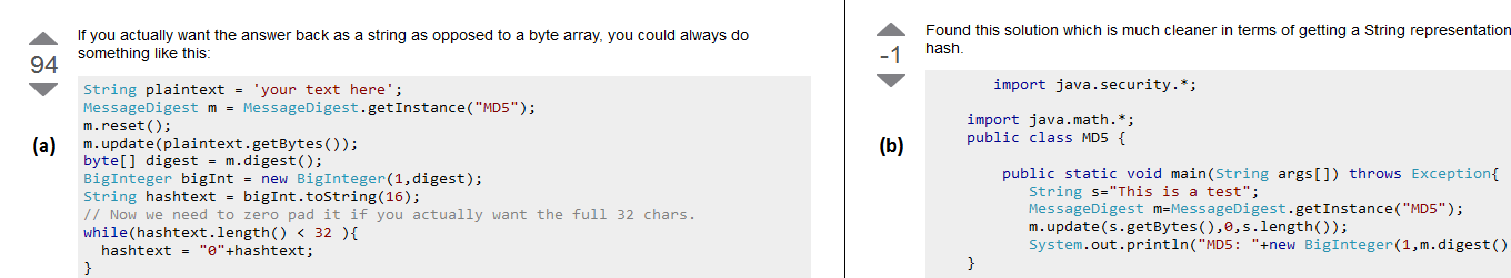
\includegraphics[width=7in ]{whole23}
\caption{(a) Promoted code example, (b) Discouraged code example}
%\label{fig_sim}
\label{fig:example}
\end{figure*}

In our research, we conduct a limited exploratory study with 110 promoted and discouraged code examples against 55 programming problems from StackOverflow. We apply four code level metrics-- readability, complexity, soundness and sonar rule compliance, and one associated metric (\eg\ author's expertise) to perceive the code level quality of those code examples, and attempt to verify against their vote score-based classification. Basically, this paper attempts to answer the following research questions.
\begin{itemize}
\item RQ1: Is the code level quality of a discouraged code example worse than that of a promoted code example?
\item RQ2: Does the metrics-based classification of StackOverflow code examples totally agree with vote score-based classification? If not, why?
\end{itemize}
While our preliminary findings with limited dataset explain the characteristics and the perceived quality of StackOverflow code examples, they must be validated with more code examples to reach a reliable conclusion.

The rest of the paper is organized as follows-- Section \ref{sec:theory}  focuses on our adopted methodology and code quality metrics, Section \ref{sec:experiment} discusses about the conducted experiments and findings, Section \ref{sec:related} describes the related works, and finally Section \ref{sec:conclusion} concludes the paper with future works.
\begin{figure}[!t]
\centering
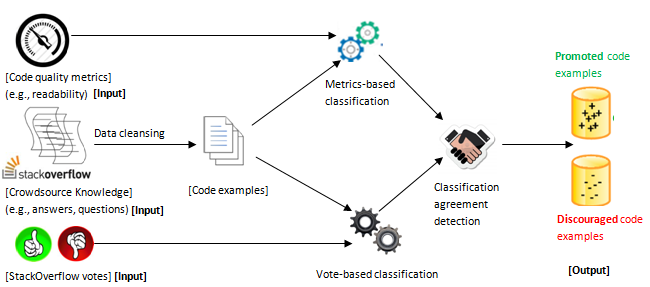
\includegraphics[width=3.5in]{sysdiag}
\caption{Schematic diagram of the proposed study}
\label{fig:sysdiag}
\end{figure}

\section{Proposed Methodology}
\label{sec:theory}
Fig. \ref{fig:sysdiag} shows the schematic diagram of our exploratory study on code quality analysis of StackOverflow code examples. In this section, we discuss about the detailed technique of the study and the metrics we use to perceive the code quality of the examples.

\subsection{Data Collection}
Given the millions of questions in StackOverflow Q \& A site from multiple programming languages and domains, we select a subset of 55 questions related to Java programming for the study. We impose certain constraints on the selection of a question--(1) The question has to be strictly related to a \emph{particular programming problem}, and the ideal answer should contain a \emph{precise and efficient code example} with comprehensive discussion, (2) Each question should have more than ten answers containing code examples to ensure that  it is a \emph{commonly discussed programming issue}. We collect the latest data dump\footnote{http://blog.stackoverflow.com/category/cc-wiki-dump/} provided under creative commons, and extract the questions and answers. Out of 82,882 questions tagged as \emph{Java}, we find 26,869 questions are strictly related to programming, and their answers contain code examples. We select a list of 75 programming questions from them, where each of the questions has more than ten answers that contain code examples. We extract the code examples from the raw HTML of StackOverflow answers against those questions, and manually analyze a random subset of the answers. We find that most of them are not directly compilable, and we perform simple tweaking (\eg\ adding import statements or semicolons, declaring undeclared variables and so on) on the examples to make them compilable. However, we find some code examples are too trivial or they cannot be compiled at all with simple tweaking, which we discard from the list. Finally, we select 55 programming questions and the representative code examples posted in their answers for the study.
\subsection{Vote Score Based Classification}
StackOverflow recognizes the technical merit and quality of a programming answer in terms of votes \cite{nasehi}, and code examples are posted as a part of the answers. While the existing studies \cite{nasehi, nier} explain their undeniable role behind the promotion and demotion of the answers, the votes cast by the large crowd of technical users for those answers can also be considered to approximate the subjective quality of the contained code examples. Given that the subjective perception of quality may vary, we choose the code examples of two extreme perceptions-- highly promoted and highly discouraged. We consider total score (\ie\ difference between up votes and down votes) and age (\ie\ difference between dumping date and post creation date) of the code examples, and calculate \emph{vote score per day} for each of them. Then, based on the scores gained per day, we choose one highly promoted and one highly discouraged code examples for each of 55 questions. The idea is to determine whether the subjective evaluation of the code example agrees with the metrics-based evaluation. We also manually analyze each code example for possible false positives, and to perceive their relative quality difference.

\subsection{Code Quality Metrics}
\label{sec:metrics}
StackOverflow code examples generally are of smaller sizes; in our case, we find them less than 15 lines in average. The code examples are posted either as complete methods or method body segments containing a few lines, and the complete class-structure are often unlikely. Therefore, most of the available code level quality metrics such as, object-oriented complexity metrics and so on, are not applicable for the code examples. Moreover, the motivation behind the quality evaluation is to determine how reusable and maintainable the code examples are for the developers. In this section, we discuss about four code related metrics used for the study.
\subsubsection{Readability (R)}
Readability of software code refers to a human judgement of how easy the code is to understand \cite{readability}. Alternatively, it also can be defined as the perceived barrier to understanding, which is essential to overcome before working with the code \cite{simpler}. Reading (\ie\ understanding) software code is the most time-consuming components of all maintenance activities \cite{readability}, and therefore, readability is directly related to software maintainability. \citet{readuse} suggest that readability also greatly contributes to reusability and portability of the code. Thus, readability is an established code quality metric, and the baseline idea is-- the more readable and understandable the code is, the easier it is to reuse and maintain in the long run. \citet{readability} propose a code readability model trained on human perception of readability or understandability. The model uses different textual source features (\eg\ length of identifiers, number of comments, line length and so on) that are likely to affect the humans' perception of readability, and then the model predicts a readability score on the scale from zero to one, inclusive, with one describing that the code is highly readable. We use the readily available library\footnote{http://www.arrestedcomputing.com/readability} by \citet{readability} to calculate the readability metric of the code examples.

\subsubsection{Author Rank (AR)}
We think that the expertise of the author of a code example is likely to influence its quality \cite{specmining}. StackOverflow provides incentives to the community users, who are actively contributing to the body of knowledge by asking important questions, posting helpful answers, adding informative comments and so on. One of those incentives is \emph{Reputation}, which is an estimated quantification of the overall contributions of a user to StackOverflow, and it can be considered as the proxy of her expertise. The idea is that a code example posted by an experienced user is likely to contain less security and performance concerns compared to that posted by an inexperienced user. \citet{specmining} use \emph{author expertise} as an indicator of code quality for specification mining, and in our study, we also use it with a focus on reusability of the code examples. To determine the rough estimate of the author expertise, we consider the reputations of all users of StackOverflow, and provide a normalized estimate on the scale from zero to one for each user, where zero describes the least experience.

\subsubsection{Code Soundness (CS)}
\citet{subjective} conduct a study on the analysis of agreement between subjective evaluation and metrics-based evaluation of software evolvability using code smells, and argue that neither technique alone is enough to detect all smells. Similarly, we can conjecture that code level metrics are not sufficient to discover all types of defects, inefficiencies or possible scopes for improvement in the code examples. StackOverflow facilitates to include the subjective evaluations for each code example in the form of comments which often contain invaluable and insightful analysis about its code quality. While one can argue that the comments are merely based on subjective viewpoints, we note that they also contain objective observations which can be considered to derive metrics describing the soundness of the code example. We leverage the objective observations to identify the strengths and weaknesses of the code example. Basically, we analyze all the comments about a code example against the code and count their numbers discussing about positive aspects (\ie\ strength) and negative aspects (\ie\ weakness) of the code. Then we normalize the \emph{strength} and \emph{weakness} measures using \emph{maximum comment count} among the code examples of the \emph{same question} as follows.
\begin{equation}
S_{i}=\frac{S_{i, count}}{max(TC_{i})},~~~ W_{i}=\frac{W_{i, count}}{max(TC_{i})}
\end{equation}
Here, $S_{i, count}, W_{i, count}$ and $TC_{i}$ denote the positive comments count, negative comments count and total comment count of a code example respectively. Both of \emph{strength} and \emph{weakness} provide a normalized score on the scale from zero to one, where zero represents the least measure of each metric. While we are not aware of if such metrics are used by any existing study, we hypothesize that they are important measures to determine the relative code quality of two code examples against the same question.

\subsubsection{Rule Violation (RV)}
Deviation from standard coding practices can be considered as an important measure to estimate the code quality of the code examples. Traditional metrics-based quality evaluation is dominated by code analysis tools, and they try to analyze the code against a certain set of recommended rules. Most of the tools concentrate on  particular aspects of code. For example, \emph{CheckStyle} focuses on conventions, \emph{PMD} on bad practices and \emph{FindBugs} focuses on potential bugs or threats. Thus, rules and standards of one tool may vary from another, and the tools are no way competitive rather than complementary. Given the facts about the tools, using any single one may not serve our purpose of detecting rule violations, and we use \emph{sonarqube}\footnote{http://www.sonarqube.org/} which combines the rules and standards of \emph{PMD, FindBugs, CheckStyles} and so on. We collect three types of violations-- critical, major and minor, in the code examples and determine \emph{violations per source line} for each of them. \citet{lochmann} propose a comprehensive quality model for a software project based on a set of rules associated with the attributes of software components and artifacts. However, given the coding structure and size of StackOverflow code examples, we hypothesize that \emph{violation per source line} is an important and credible metric to estimate the relative quality of the code examples.  

\subsection{Metrics Based Evaluation}
In our study, we focus on the quality analysis of StackOverflow code examples with the notion of their reusability. Given the developing interests of the community on the posted code examples \cite{nasehi, nier}, the idea of investigating into their code quality using available metrics, is quite intriguing to us. We consider the readability, adherence to the best practices and identified issues or threats in the code examples to estimate their quality for reusability. One can argue that complexity can be a useful metric for this purpose. However, given the size and structure of the code examples, object-oriented complexity metrics (\eg\ CK metrics) or cyclomatic complexity are not usefully applicable, and we believe that the discussed metrics (in Section \ref{sec:metrics}) are the most contributing factors towards reusability of the StackOverflow examples. While other metrics contribute to the code quality positively, \emph{weakness} and \emph{rule violation} metrics perform negatively. We manually analyze 50 code examples and label them either as \emph{promoted} or \emph{discouraged}. Then we use those labeled code examples along with their computed metrics (\ie\ Section \ref{sec:metrics}), and use logistic regression to determine their relative predictive power (\ie\ Odds ratios). Finally, we get the following quality model to perform the relative quality analysis among the code examples, where the coefficients are the predictive power (\ie\ importance) of corresponding metrics.
\begin{equation}\label{eq:model}
\begin{split}
Q_{i}=3.0043\times R_{i}+0.0454\times AR_{i}
+8.04884\times S_{i}\\+0.5078\times W_{i}+0.1547\times RV_{i}
\end{split}
\end{equation}
In the model, we find \emph{readability} and \emph{strength} as the most dominating features, whereas \emph{author rank} has the least influence in predicting code quality, which refutes our initial assumption about it.

\section{Results and Discussions}
\label{sec:experiment}
In our experiment, we use the quality model to estimate the quality measures of 110 code examples against 55 programming questions \cite{expdata}. It should be noted that we use the estimates to perform the comparative quality analysis among the code examples of the same question. The idea is to determine whether a code example promoted by StackOverflow is actually of better code quality than the one which is discouraged by StackOverflow. Table \ref{table:result} shows the results of our preliminary experiments., where the metric-based relative quality prediction agrees with that of StackOverflow at best for 41(74.54\%)  out of 55 questions. It also shows the results for different combination of metrics, and the empirical findings shows that \emph{readability} and \emph{strength} of code examples are the most effective metrics for relative quality analysis. In the next section, we attempt to answer our research questions.

\emph{RQ1: Is the code level quality of a discouraged code example worse than that of a promoted code example?} The preliminary results show that it is true for 74.54\% code examples of the dataset. \emph{Readability}, \emph{strength} and \emph{weakness} metrics are greatly related to easier comprehension, efficiency, security and maintainability and other attributes (\ie\ quality) of the software code that stimulate its reuse \cite{readability}, and we also found those metrics promising in our experiment for quality analysis. Basically, our model performs better when those metrics can be calculated properly from the available information, especially \emph{strength} and \emph{weakness} metrics which are derived from the conversations (\ie\ comments) among the community users followed by the code example. Given the challenges of extracting metrics from text, they really help in code quality analysis if they can be extracted properly. So, to answer the first question, the discouraged code examples are of inferior quality to promoted code examples most of the time; however, this can be verfied with the availability of essential and reliable information.

\emph{RQ2: Does the metrics-based classification of StackOverflow code examples totally agree with vote score-based classification? If not, why?} The two classifications agree mostly, about 75\%; however, the complete agreement may not be possible. We investigate into the 14 cases (28 code examples and their metrics) for which our quality model does not match with StackOverflow, and find a few issues or scenarios. First, most of them do not contain comments given that metrics from the comments play major parts in our model, and the model does not perform well for those cases. Second, our model does not use any threshold to describe a code example either as promoted or discouarged, rather it uses relative quality analysis which may not effective all the time. For example, if there is little difference in the quality estimate of two code examples, the model still identifies the promoted and discouraged one; however, actully both of them should be considered as promoted or discouarged. Third, StackOverflow contains some code examples, which are highly simplified with little technical merit, and are often intended for student homeworks and preliminary learning, and they are also highly voted. Our model does not perform well in that case. Fourth, we also find some cases where \emph{vote score} does not necessarily represent the evaluation of the contained code examples or they do not play major part in answering the question.

\begin{table}
\label{table:result}
\centering
\caption{Experimental Results}
\begin{tabular}{l|c|c|c}
\hline
\textbf{Metrics} & \textbf{APC} & \textbf{A} & \textbf{D}\\
\hline
\{R\} & 25(55) & 45.45\% & 54.55\%\\
\hline
\{R, S\} & 38(55) & 69.09\% & 30.90\%\\
\hline
\{R, S, W\} & 41(55) & 74.54\% & 25.45\% \\
\hline
\{R, S, W, RV\} & 40(55) & 72.72\% & 27.27\% \\
\hline
\{R, S, W, AR\} &  41(55) & 74.54\% & 25.45\% \\
\hline
\{R, S, W, RV, AR\} & 41(55) & \textbf{74.54\%} & \textbf{25.45\%} \\
\hline\end{tabular}
\end{table}




\section{Related Works}
\label{sec:related}
Existing studies focus on software code metrics for checking readability \cite{readability, simpler}, reusability \cite{reusability}, effectiveness of refactoring \cite{refactoring} and comprehensive quality \cite{ijert, lochmann, survey, foss, oss} of the software code. Our work is closely related to the comparative analysis between subjective and metrics based evaluation of software evolvability by \citet{subjective} as we have a similar goal with different methodology and subject system. Two existing studies \cite{nasehi, nier} explain the role of code examples in StackOverflow question or answer post; however, to our knowledge, this is the first attempt to analyze the subjective and metrics based code quality of the code examples, and to determine their agreement.


\section{Conclusion \& Future Works}
\label{sec:conclusion}
To summarize, given the developing interest of StackOverflow community to the code examples, we attempt to determine whether their subjective evaluation by the community agrees with the metrics-based evaluation. We conduct an exploratory study with 110 representative code examples against 55 programming questions, and develop a code quality analysis model with the available and applicable metrics. The model agrees with StackOverflow in relative quality prediction for 74.54\% code examples, which is quite promising and revealing about the effectiveness of StackOverflow votes. However, the finding must be extensively validated with more code examples from Java programming and other languages or domains to the answer the research questions properly.







% The following two commands are all you need in the
% initial runs of your .tex file to
% produce the bibliography for the citations in your paper.
\bibliographystyle{plainnat}
\scriptsize
\bibliography{sigproc}  % sigproc.bib is the name of the Bibliography in this case
% You must have a proper ".bib" file
%  and remember to run:
% latex bibtex latex latex
% to resolve all references
%
% ACM needs 'a single self-contained file'!
%
%APPENDICES are optional
%\balancecolumns
\end{document}
